\section{Evaluation}
We analyze over 3,000,000 SCOPE jobs that run on five data centers at Microsoft. In summary, our experiments illustrate the following:

\begin{itemize}
\item \emph{What is the proportion of time spent in native vs. non-native job vertices?} Between \nonNativeTimeL{} and \nonNativeTimeU \% of data center time is spent in job vertices that run managed code.

\item \emph{What proportion of time can be optimized having the current list of methods with C++ implementation?} With the current list of intrinsicable methods we can optimize up to \optimizableU{} \% of data center time.

\item \emph{What proportion of time can be optimized by extending the list of methods with C++ implementation? Which methods should be the most important for C++ implementation?}
By increasing the list of intrinsics and optimizing all inlineable methods we can optimize up to \potentiallyOptimizableU{} \% of data center time. Furthermore, we conclude that \emph{String} methods are the most important .NET framework methods amenable for C++ implementations.


\end{itemize}

\subsection{Experimental Setup}
To understand performance bottlenecks in SCOPE jobs we analyze over 3,000,000 jobs across 5 data centers. Table~\ref{tb:projects} lists for every data center, the number of analyzed jobs along with their CPU time measured in hours. We observe that number of jobs and CPU time significantly vary between data centers. For example, data center \emph{cosmos15} run the highest proportion of jobs we analyze, while \emph{cosmos9} run the most expensive jobs. This is expected because different data centers are usually tailored for different types of jobs. 


\begin{table}[ht]
\centering
\begin{tabular}{lrr}

  Data center & Number of jobs & CPU time (in hours) \\
 \midrule
cosmos8 & 375,974 & 28,559,063 \\
cosmos9 & 171,203 & 40,714,052 \\
cosmos11 & 851,222 & 23,312,271\\
cosmos14 & 474,911 & 21,299,039\\
cosmos15 & 1,200,026 & 31,324,407 \\
\midrule
Total: & 3,073,336 & 145,208,834\\
\midrule

\end{tabular}
 \label{tb:projects}
 \caption{Analyzed jobs and their CPU time}
\end{table}




\subsection{Native vs. Non-Native Time}
Before optimizing non-relational logic in SCOPE jobs, it is important to understand how much time is spent in job vertices that run non-relational code. The analysis of C++ code returns for every job vertex whether it runs as native or managed code. Combined with data from \emph{Runtime Statistics} we also find how much time is taken by every job vertex.

Figure~\ref{fig:nativeVsNonNative} illustrates our results. It shows for every data center how much time is spent in native and non-native vertices. Grey area denotes few exceptional vertices for which the analysis can not certainly distinguish the code that runs inside a vertex. For example, sometimes the analysis does not detect any source of managed code in a vertex that supposedly runs C\# code. The time of such vertices we assign to gray area.

We conclude from Figure~\ref{fig:nativeVsNonNative} that time spent in non-native code represents a large fraction of data center time. For example, in cosmos9, the time spent in native vertices contributes to only 21.30\% of data center time. These results illustrate the potential of optimizing the non-relational code and it influence on data center time.

\begin{figure*}[ht]
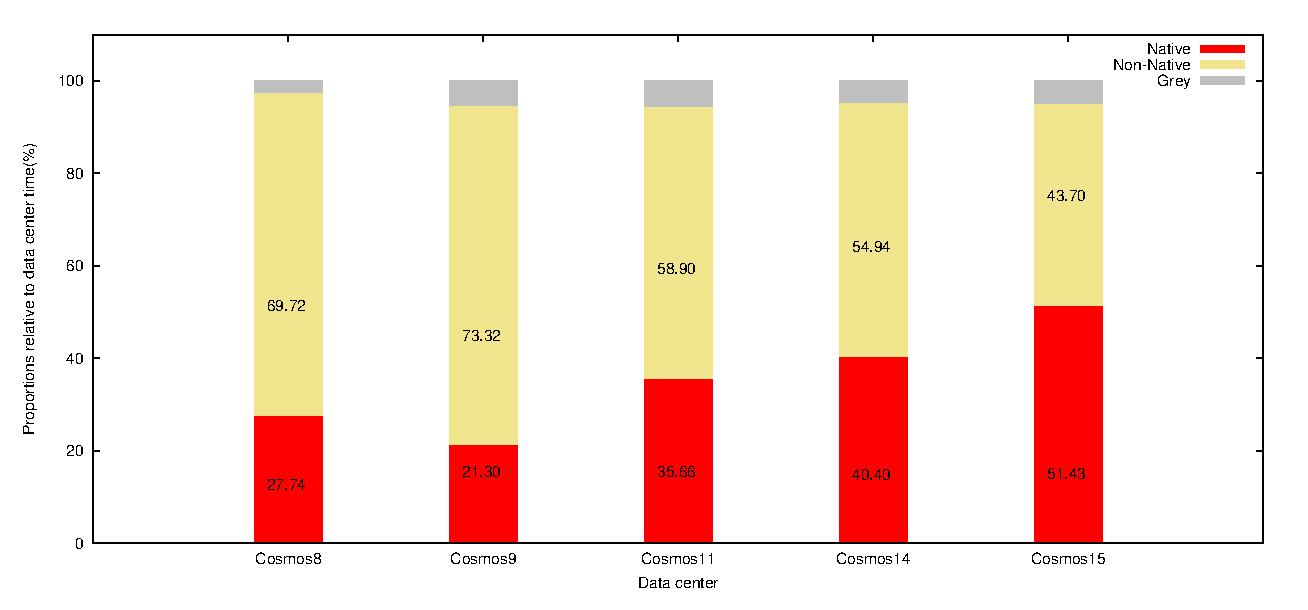
\includegraphics[scale = 0.7]{graphs/proportions}
\caption{Time spent in native vs. non-native vertices}
\label{fig:nativeVsNonNative}
\end{figure*}

\subsection{Optimizable Job Stages}

This figure illustrates how much time is spent in job stages that we can optimize by inlining the user-written logic. X axis represents data center, Y axis represents precentage of time spent in inlineable job stages relative to total data center time and total time spent in non-native code.

\begin{figure}[ht]
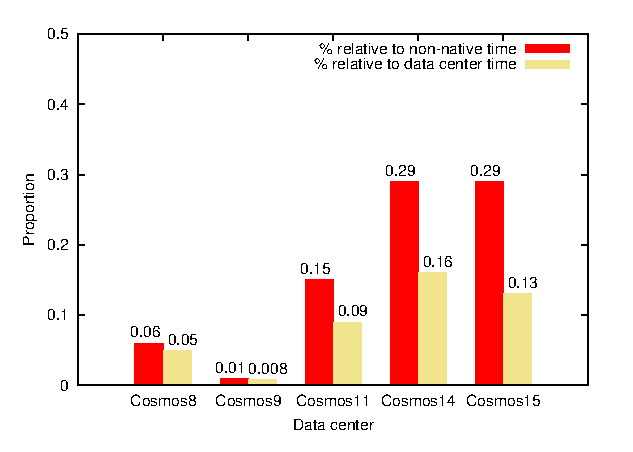
\includegraphics[scale=0.8]{graphs/optimizable}
\caption{Optimizable job vertices}
\end{figure}

\subsection{Potential for C++ Translation}

The following figure shows how much time can be affected by extending the list of functions that have C++ implementations. X axis represents data center, Y axis precentage of time spent in job stages that can be optimized, relative to total non-native and data center time.

\begin{figure}[ht]
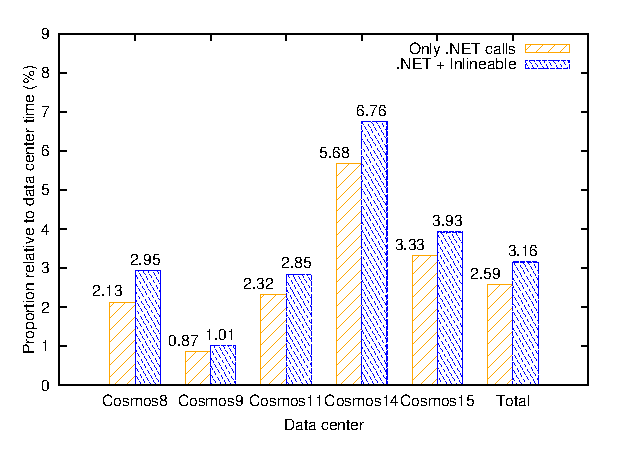
\includegraphics[scale=0.8]{graphs/potentiallyOptimizable}

\caption{Potentially optimizable job vertices}
\end{figure}

\subsubsection{Most Relevant .NET Framework Methods}

Ranking criteria: cost of job stage
\begin{table*}[ht]
\small
 \begin{tabular}{@{}llllp{3.5cm}@{}}

  Cosmos8 & Cosmos9 & Cosmos11 & Cosmos14 & Cosmos15 \\
 \midrule
System.Convert.ToInt64 & \textbf{System.String.Equals} & System.String.Replace & \textbf{System.DateTime.ToString} & \textbf{System.String.ToLower} \\
System.Int32.Parse & \textbf{System.String.ToLower} & \textbf{System.String.ToLower} & System.String.IndexOf & System.String.LastIndexOf \\
\textbf{System.String.ToLower} & System.Int32.Parse & System.String.ToUpper & System.DateTime.ToLocalTime & \textbf{System.DateTime.ToString}\\
\textbf{System.String.Concat} & System.String.Replace & \textbf{System.String.Concat} & \textbf{System.String.ToLower} & \textbf{System.String.Concat}\\
System.String.Replace & System.Convert.ToDateTime & System.String.Trim & System.String.ToUpper & System.Convert.ToUInt64 \\
System.Double.Parse & System.Regex.isMatch & System.Math.Max & System.Regex.IsMatch & System.Enumerable.SelectMany \\
System.Math.Round& System.DateTime.ToUniversalTime & \textbf{System.String.Equals} & \textbf{System.String.Equals} & System.Enumerable.Distinct \\
System.Char.NewArr & \textbf{System.String.Concat} & System.TimeSpan.Days & \textbf{System.String.Concat} & System.String.Format \\
System.String.ToUpper & System.TimeSpan.Days & \textbf{System.DateTime.ToString} & System.String.Trim & \textbf{System.String.Equals}\\
System.String.Upper & System.DateTime.Subtract & System.String.ToCharArray & System.String.Split & System.String.IndexOf \\

\midrule
1.27\%\footnote{proportion relative to data center time} & 0.63\% & 1.61\% & 5.15\% & 1.8\%\\
\midrule

\end{tabular}
 \label{tb:projects}
\caption{Most relevant .NET Framework methods per data center. Methods in bold are those that appear in the top 10 for at least three data centers.}
\end{table*}

The table below shows for every data center what are the most important .NET framework methods taking into account our ranking criteria...Furthermore, it illustrates how much time would be affected by providing C++ implementation of these methods, relative to total non-native time and total data center time.

\begin{figure}[ht]
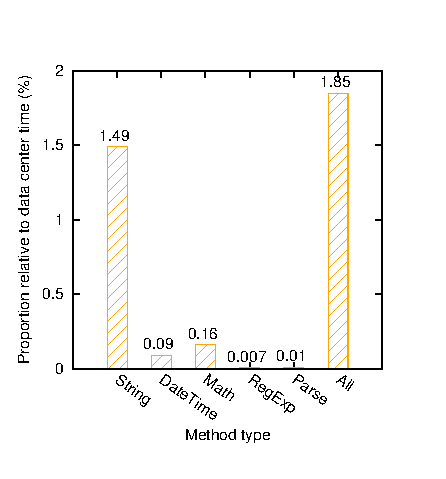
\includegraphics{graphs/methodTypes}
\caption{Relevance of .NET framework method types (cosmos11)}
\label{fig:methodTypes}
\end{figure}








